\documentclass[10pt]{beamer}

% Packages
\usepackage[utf8]{inputenc}
\usepackage[T1]{fontenc}
\usepackage{amsmath, amssymb, amsthm}
\usepackage{graphicx}
\usepackage{booktabs}
\usepackage{hyperref}
\usepackage{tikz}
\usetikzlibrary{shapes,arrows,positioning,calc}

% Theme settings
\usetheme{default}
\usecolortheme{default}
\usefonttheme{professionalfonts}

\definecolor{ImperialBlue}{RGB}{0, 62, 116}
\definecolor{DarkGray}{RGB}{51, 51, 51}
\definecolor{LightGray}{RGB}{245, 245, 245}
\definecolor{AccentOrange}{RGB}{214, 96, 77}
\definecolor{AccentGreen}{RGB}{46, 139, 87}

% Apply colors
\setbeamercolor{frametitle}{fg=ImperialBlue, bg=white}
\setbeamercolor{title}{fg=ImperialBlue}
\setbeamercolor{structure}{fg=ImperialBlue}
\setbeamercolor{normal text}{fg=DarkGray}
\setbeamercolor{block title}{fg=white, bg=ImperialBlue}
\setbeamercolor{block body}{fg=DarkGray, bg=LightGray}
\setbeamercolor{itemize item}{fg=ImperialBlue}
\setbeamercolor{enumerate item}{fg=ImperialBlue}

% Remove navigation symbols
\setbeamertemplate{navigation symbols}{}

% Customize frame title
\setbeamertemplate{frametitle}{
  \vspace{0.5em}
  \insertframetitle
  \vspace{0.3em}
}

% Customize itemize
\setbeamertemplate{itemize items}[circle]
\setlength{\leftmargini}{1.5em}

% Footer
\setbeamertemplate{footline}{
  \leavevmode%
  \hbox{%
  \begin{beamercolorbox}[wd=.333333\paperwidth,ht=2.25ex,dp=1ex,left]{author in head/foot}%
    \hspace{1em}\usebeamerfont{author in head/foot}\insertshortauthor
  \end{beamercolorbox}%
  \begin{beamercolorbox}[wd=.333333\paperwidth,ht=2.25ex,dp=1ex,center]{title in head/foot}%
    \usebeamerfont{title in head/foot}\insertshorttitle
  \end{beamercolorbox}%
  \begin{beamercolorbox}[wd=.333333\paperwidth,ht=2.25ex,dp=1ex,right]{date in head/foot}%
    \usebeamerfont{date in head/foot}\insertshortdate{}\hspace*{2em}
    \insertframenumber{} / \inserttotalframenumber\hspace*{2ex} 
  \end{beamercolorbox}}%
  \vskip0pt%
}

% Commands for highlighting
\newcommand{\emphbox}[1]{\colorbox{LightGray}{\textcolor{DarkGray}{#1}}}
\newcommand{\highlight}[1]{\textcolor{AccentOrange}{\textbf{#1}}}
\newcommand{\good}[1]{\textcolor{AccentGreen}{#1}}
\newcommand{\bad}[1]{\textcolor{AccentOrange}{#1}}

%----------------------------------------------------------------------------------------
\title{Blockchain in Traditional Finance}
\subtitle{ECOM215: Blockchain Economics and Digital Assets}
\author{Dr Daniele Bianchi}
\institute{Queen Mary, University of London}
\date{Semester B, 2025/2026}
%----------------------------------------------------------------------------------------

\begin{document}

\AtBeginSection[]{
  \begin{frame}[plain]
    \vfill
    \begin{center}
      {\Large\color{ImperialBlue}\insertsection}
    \end{center}
    \vfill
  \end{frame}
}

\begin{frame}[plain]
  \titlepage
\end{frame}

\begin{frame}{Today's Agenda}
  \tableofcontents
\end{frame}

%----------------------------------------------------------------------------------------
\section{Why Traditional Finance Cares About Blockchain}
%----------------------------------------------------------------------------------------

\begin{frame}{A Different Conversation}
  Weeks 1--8 largely focused on \highlight{crypto-native} applications: DeFi, stablecoins, NFTs, and cryptocurrency investment.
  
 \vspace{1em}
   This week is about something different: can blockchain technology improve the \highlight{existing financial system}---the infrastructure used by banks, exchanges, and central banks to move money and securities around the world?
  
  \vspace{1em}
  \textbf{The core idea}: Financial infrastructure is old, slow, and expensive. Many processes that should take seconds---settling a stock trade, sending money abroad, verifying ownership of a bond---instead take days and involve multiple intermediaries, each adding cost and risk.
  
  \vspace{1em}
  \textbf{The pitch from blockchain}: Replace some of these intermediaries with shared ledgers and smart contracts that settle transactions faster, with fewer parties, and at lower cost.
  
  \vspace{1em}
  \highlight{The question we need to answer}: How much of this is real, and how much is marketing?
\end{frame}

\begin{frame}{What is ``Financial Infrastructure''?}
  Before we discuss how blockchain might improve financial infrastructure, we need to understand what it is.
  
  \vspace{1em}
  \highlight{Financial infrastructure} refers to the systems and institutions that make financial transactions possible. Key components:
  \begin{itemize}
    \item \textbf{Payment systems}: How money moves from one bank account to another (e.g., CHAPS in the UK, Fedwire in the US, SWIFT for international messaging)
    \item \textbf{Securities settlement}: How ownership of shares and bonds is transferred after a trade (e.g., CREST in the UK, DTCC in the US)
    \item \textbf{Clearing houses}: Institutions that sit between buyer and seller to guarantee that both sides honour the trade
    \item \textbf{Custodians}: Banks that hold assets on behalf of investors and keep track of who owns what
  \end{itemize}
  
  \vspace{1em}
  Most of this infrastructure was built in the 1970s--1990s and has been incrementally updated since. It works, but it is complex, expensive, and slow by modern standards.
\end{frame}

\begin{frame}{The Cost of Financial Infrastructure}
  \textbf{Why does it matter that settlement takes a day or two?}
  
  \vspace{1em}
  Every hour between a trade and its final settlement creates risk and cost:
  \begin{itemize}
    \item \textbf{Counterparty risk}: Between trade and settlement, either party could default. The longer the gap, the greater the exposure.
    \item \textbf{Capital requirements}: Regulators require banks and brokers to hold capital against unsettled trades. Faster settlement = less capital tied up = more efficient use of resources.
    \item \textbf{Operational cost}: Multiple intermediaries (brokers, clearing houses, depositories, custodians) each maintain their own records. Reconciling these records is expensive and error-prone.
    \item \textbf{Failed trades}: When records don't match, trades ``fail'' and must be corrected manually. This is surprisingly common.
  \end{itemize}
  
  \vspace{0.5em}
  \textbf{Scale of the problem}: Global post-trade costs are estimated at \$15--20 billion per year. The question is how much of this could be reduced.
\end{frame}

%----------------------------------------------------------------------------------------
\section{Settlement and Clearing: How It Works Today}
%----------------------------------------------------------------------------------------

\begin{frame}{What Happens When You Buy a Share?}
  Suppose you place an order to buy 100 shares of Vodafone through your broker. What happens next?
  
  \vspace{0.5em}
  \textbf{Step 1: Execution.} Your broker finds a seller (or a market maker) on the London Stock Exchange. The trade is \textit{agreed}---but nothing has actually moved yet.
  
  \vspace{0.5em}
  \textbf{Step 2: Clearing.} The trade is sent to a \highlight{clearing house} (in the UK, LCH or the LSE's own clearing service). The clearing house becomes the buyer to every seller and the seller to every buyer. Its purpose: if your counterparty goes bankrupt before settlement, the clearing house guarantees the trade.
  
  \vspace{0.5em}
  \textbf{Step 3: Settlement.} On the \highlight{settlement date}---currently one business day after the trade (T+1 in the US since May 2024, with the UK and EU planning a move to T+1 in 2027)---the actual exchange happens. Your cash is debited, the seller's cash is credited, and ownership of the shares is transferred.
  
  \vspace{0.5em}
  \textbf{Step 4: Custody.} Your broker (or a custodian bank) holds the shares on your behalf and maintains the record of your ownership.
\end{frame}

\begin{frame}{What is T+1 and Why Does It Exist?}
  \highlight{T+1} means that the trade settles one business day after execution. Until May 2024, the US used T+2 (two business days).
  
  \vspace{0.5em}
  \textbf{Why not settle instantly?}
  \begin{itemize}
    \item \textbf{Netting}: Clearing houses wait until the end of the day to calculate net positions. If Bank A owes Bank B \pounds 10 million and Bank B owes Bank A \pounds 8 million, only \pounds 2 million actually moves. This massively reduces the amount of cash and securities that need to change hands.
    \item \textbf{Error correction}: The delay gives parties time to catch and fix mistakes before settlement is final.
    \item \textbf{Funding}: Buyers need time to arrange payment; sellers need time to locate and deliver securities.
    \item \textbf{Time zones}: When a trade involves parties in London and Tokyo, coordinating same-day settlement is logistically challenging.
  \end{itemize}
  
  \vspace{0.5em}
  \begin{block}{Important Nuance}
  If settlement were truly instant, \textit{every} trade would require full gross payment. This could actually \highlight{increase} liquidity demands rather than reduce them. Blockchain advocates sometimes overlook this.
  \end{block}
\end{frame}

\begin{frame}{What Blockchain Could Change}
  \textbf{The promise:}
  \begin{itemize}
    \item \textbf{Atomic settlement}: Cash and securities move simultaneously on a shared ledger. If one leg fails, neither executes. This eliminates settlement risk by design.
    \item \textbf{Single source of truth}: All parties see the same ledger. No reconciliation needed between separate databases.
    \item \textbf{Programmable compliance}: Smart contracts can enforce transfer restrictions, KYC requirements, and regulatory rules automatically.
  \end{itemize}
  
  \vspace{0.5em}
  \textbf{The reality check:}
  \begin{itemize}
    \item \bad{Netting benefits are lost} if every trade settles individually in real time
    \item \bad{Legal finality} is not automatic: Laws differ by jurisdiction and most do not yet recognise on-chain settlement as legally final.
    \item \bad{Interoperability}: The new system must connect to existing infrastructure during any transition---banks cannot switch overnight.
    \item \bad{Governance}: Who runs the shared ledger? A consortium? A public chain? Each option raises different trust and control issues.
  \end{itemize}
\end{frame}

\begin{frame}{The Netting Problem: A Worked Example}
  \textbf{Without netting} (gross settlement):
  
  \vspace{0.3em}
  Suppose three banks each trade with each other during a day:
  \begin{center}
    \small
    \begin{tabular}{lccc}
      \toprule
      \textbf{Trade} & \textbf{From} & \textbf{To} & \textbf{Amount} \\
      \midrule
      1 & Bank A & Bank B & \pounds 100m \\
      2 & Bank B & Bank C & \pounds 80m \\
      3 & Bank C & Bank A & \pounds 60m \\
      4 & Bank B & Bank A & \pounds 70m \\
      \midrule
      \multicolumn{3}{l}{\textbf{Total gross flows}} & \textbf{\pounds 310m} \\
      \bottomrule
    \end{tabular}
  \end{center}
  
  \vspace{0.5em}
  \textbf{With netting}: The clearing house calculates net positions: A owes \pounds 30m net to B, B owes \pounds 10m net to C, C owes \pounds 60m net to A. \textbf{Total net flows: \pounds 100m}---less than one-third of the gross amount.
  
  \vspace{0.5em}
  \textbf{Implication}: Instant gross settlement on a blockchain would require banks to have \pounds 310m in liquidity ready, rather than \pounds 100m. This is a real economic cost that must be weighed against faster settlement.
\end{frame}

%----------------------------------------------------------------------------------------
\section{Institutional Blockchain Initiatives}
%----------------------------------------------------------------------------------------

\begin{frame}{Who is Building What?}
  Major financial institutions are not waiting for public blockchains to mature. They are building their own systems---mostly on \highlight{permissioned} (private) blockchains where only approved participants can join.
  
  \vspace{1em}
  \textbf{Key distinction from public blockchains (Ethereum, Bitcoin):}
  \begin{itemize}
    \item Access is restricted to known, vetted participants
    \item No cryptocurrency or token speculation
    \item Consensus is simpler (no mining or staking---participants are trusted)
    \item Regulatory compliance is built in from the start
    \item But: less decentralised, less composable, less open
  \end{itemize}
  
  \vspace{1em}
  We will examine four major initiatives. For each, we ask: What problem does it solve? What has actually been deployed? And what are the limitations?
\end{frame}

\begin{frame}{JPMorgan Kinexys (formerly Onyx)}
  \highlight{Kinexys} is JPMorgan's blockchain platform, one of the most advanced institutional deployments.
  
  \vspace{0.5em}
  \textbf{What it does:}
  \begin{itemize}
    \item \textbf{JPM Coin}: A digital token representing US dollars used for instant, 24/7 interbank payments between JPMorgan clients. Each token is backed 1:1 by dollar deposits.
    \item \textbf{Intraday repo}: Short-term borrowing and lending settled on-chain. Clients can borrow against Treasury collateral and repay within hours, rather than overnight.
  \end{itemize}
  
  \vspace{0.5em}
  \textbf{Scale}: Processes approximately \$2 bn/day in transactions (as of 2024).
  
  \vspace{0.5em}
  \textbf{Honest assessment:}
  \begin{itemize}
    \item \good{Real product}, used by real clients, processing real money
    \item \bad{Closed system}: Only works for JPMorgan clients. Not interoperable with other banks' systems.
    \item \bad{Centralised}: JPMorgan controls the ledger. The economic benefit is incremental---faster settlement within one bank's network---not transformative.
  \end{itemize}
\end{frame}

\begin{frame}{DTCC Digital Securities Management}
  The \highlight{Depository Trust \& Clearing Corporation (DTCC)} is the backbone of US securities settlement. It processes virtually all US equity and bond trades.
  
  \vspace{0.5em}
  \textbf{What DTCC is doing:}
  \begin{itemize}
    \item \textbf{Project Ion}: A blockchain-based alternative settlement system for US equities, running in parallel with the existing system since 2022.
    \item \textbf{Digital Securities Management (DSM)}: Infrastructure for issuing, transferring, and settling tokenized securities on a distributed ledger.
  \end{itemize}
  
  \vspace{0.5em}
  \textbf{Why it matters}: If the entity that already settles all US equities adopts blockchain, the impact is far greater than any bank doing it alone.
  
  \vspace{0.5em}
  \textbf{Honest assessment:}
  \begin{itemize}
    \item \good{Credibility}: DTCC is the incumbent provider---its adoption signals that blockchain is taken seriously at the highest levels.
    \item \bad{Cautious pace}: Project Ion has been in pilot for years with limited throughput. Full migration is not imminent.
    \item The biggest question: Will blockchain \textit{replace} DTCC's existing system, or simply be absorbed as an internal upgrade? 
  \end{itemize}
\end{frame}

\begin{frame}{Canton Network and Fnality}
  \textbf{Canton Network}:
  \begin{itemize}
    \item A \highlight{privacy-preserving} blockchain network designed for institutional finance
    \item Founded by Digital Asset (a fintech company); participants include Goldman Sachs, BNP Paribas, Deloitte, and others
    \item Key feature: Participants can transact with each other without revealing their data to other network members---essential for banks with confidentiality requirements
  \end{itemize}
  
  \vspace{0.5em}
  \textbf{Fnality}:
  \begin{itemize}
    \item A consortium of 17 major banks (including Barclays, UBS, Santander, CIBC) building a \highlight{utility settlement coin (USC)}---a digital token backed by central bank reserves
    \item Purpose: Provide a ``cash leg'' for on-chain settlement of securities and derivatives
    \item The problem it solves: You can tokenize a bond, but if the cash payment still goes through traditional banking, you haven't really improved settlement.
  \end{itemize}
  
\end{frame}

\begin{frame}{Reality Check: What Has Actually Shipped?}
  \begin{center}
    \small
    \begin{tabular}{p{2.5cm}p{2.5cm}p{2cm}p{2.5cm}}
      \toprule
      \textbf{Initiative} & \textbf{What it does} & \textbf{Status} & \textbf{Limitation} \\
      \midrule
      JPMorgan Kinexys & Interbank payments, intraday repo & Live (\$2bn/day) & Closed to JPM clients \\
      \addlinespace
      DTCC Ion / DSM & Equity settlement, tokenized securities & Pilot & Limited throughput \\
      \addlinespace
      Canton Network & Privacy-preserving institutional DeFi & Early deployment & Few live transactions \\
      \addlinespace
      Fnality (USC) & Cash settlement token backed by CB reserves & Approved, building & Not yet at scale \\
      \addlinespace
%      BlackRock BUIDL & Tokenized T-bills on Ethereum & Live (\$500m+) & Qualified purchasers only \\
      \bottomrule
    \end{tabular}
  \end{center}
  
  \vspace{0.3em}
  \textbf{Pattern}: The initiatives that are actually live tend to be narrow in scope and centralised. The broader, more ambitious visions remain in pilot or early stages.
  
\end{frame}

%----------------------------------------------------------------------------------------
\section{Wholesale CBDCs and Cross-Border Payments}
%----------------------------------------------------------------------------------------

\begin{frame}{The Cross-Border Payments Problem}
  Sending money internationally is slow, expensive, and opaque. To understand why, you need to know how it currently works.
  
  \vspace{0.5em}
  \textbf{The \highlight{correspondent banking} model}:
  
  \vspace{0.5em}
  Suppose a UK company wants to pay a supplier in Japan. The UK company's bank (Barclays) probably does not have a direct relationship with the supplier's bank (MUFG). Instead:
  \begin{enumerate}
    \item Barclays sends a \textbf{SWIFT message} (an instruction, not a payment) to a bank in Japan it does have a relationship with.
    \item The correspondent bank forwards the payment to MUFG.
    \item Each bank in the chain deducts a fee and may take a day to process.
  \end{enumerate}
  
  \vspace{0.5em}
  \textbf{Result}: A payment that should take seconds involves 2--5 intermediary banks, takes 2--5 business days, costs 1--5\% of the transaction value, and offers limited visibility on where the money is at any given moment.
  
  \vspace{0.5em}
  \highlight{SWIFT} is not a payment system---it is a \textit{messaging} network. It tells banks what to do, but the actual money movement happens through a chain of accounts.
\end{frame}

\begin{frame}{What is a Wholesale CBDC?}
  In Week 5, we discussed \highlight{retail CBDCs}---digital money issued by a central bank for use by the general public (households and businesses).
  
  \vspace{0.5em}
  A \highlight{wholesale CBDC} is different: it is digital central bank money available only to \textbf{financial institutions}---banks, clearing houses, and other regulated entities.
  
  \vspace{0.5em}
  \textbf{Why is this useful?}
  \begin{itemize}
    \item Banks already hold reserves at the central bank, but these reserves operate on legacy systems with limited hours and slow processing.
    \item A wholesale CBDC would represent central bank reserves as \textbf{digital tokens on a shared ledger}, enabling faster, programmable, and potentially 24/7 interbank settlement.
    \item A wholesale CBDC provides a \textit{tokenized cash leg} that settles simultaneously with the tokenized security.
  \end{itemize}
  
  \vspace{0.3em}
  \begin{block}{Key Point}
    Wholesale CBDCs are less controversial than retail CBDCs because they don't change the relationship between citizens and the central bank.
  \end{block}
\end{frame}

\begin{frame}{Cross-Border CBDC Experiments}
  Several central bank experiments are testing whether wholesale CBDCs can fix cross-border payments.
  
  \vspace{0.3em}
  \textbf{Project mBridge} (BIS, PBOC, HKMA, Bank of Thailand, Central Bank of UAE):
  \begin{itemize}
    \item A shared platform where participating central banks issue their own wholesale CBDCs
    \item Banks can exchange currencies directly on the platform, bypassing correspondent banking
    \item Reached ``minimum viable product'' stage in 2024
    \item Potential to dramatically reduce cost/time of cross-border payments
  \end{itemize}
  
  \vspace{0.3em}
  \textbf{Project Dunbar} (BIS, Reserve Bank of Australia, Bank Negara Malaysia, Monetary Authority of Singapore, South African Reserve Bank):
  \begin{itemize}
    \item Tested shared platform for multi-CBDC settlement
    \item Demonstrated that direct transfers between currencies are technically feasible
  \end{itemize}
  
\end{frame}

\begin{frame}{Cross-Border CBDC Experiments}
  \begin{figure}
    \centering
    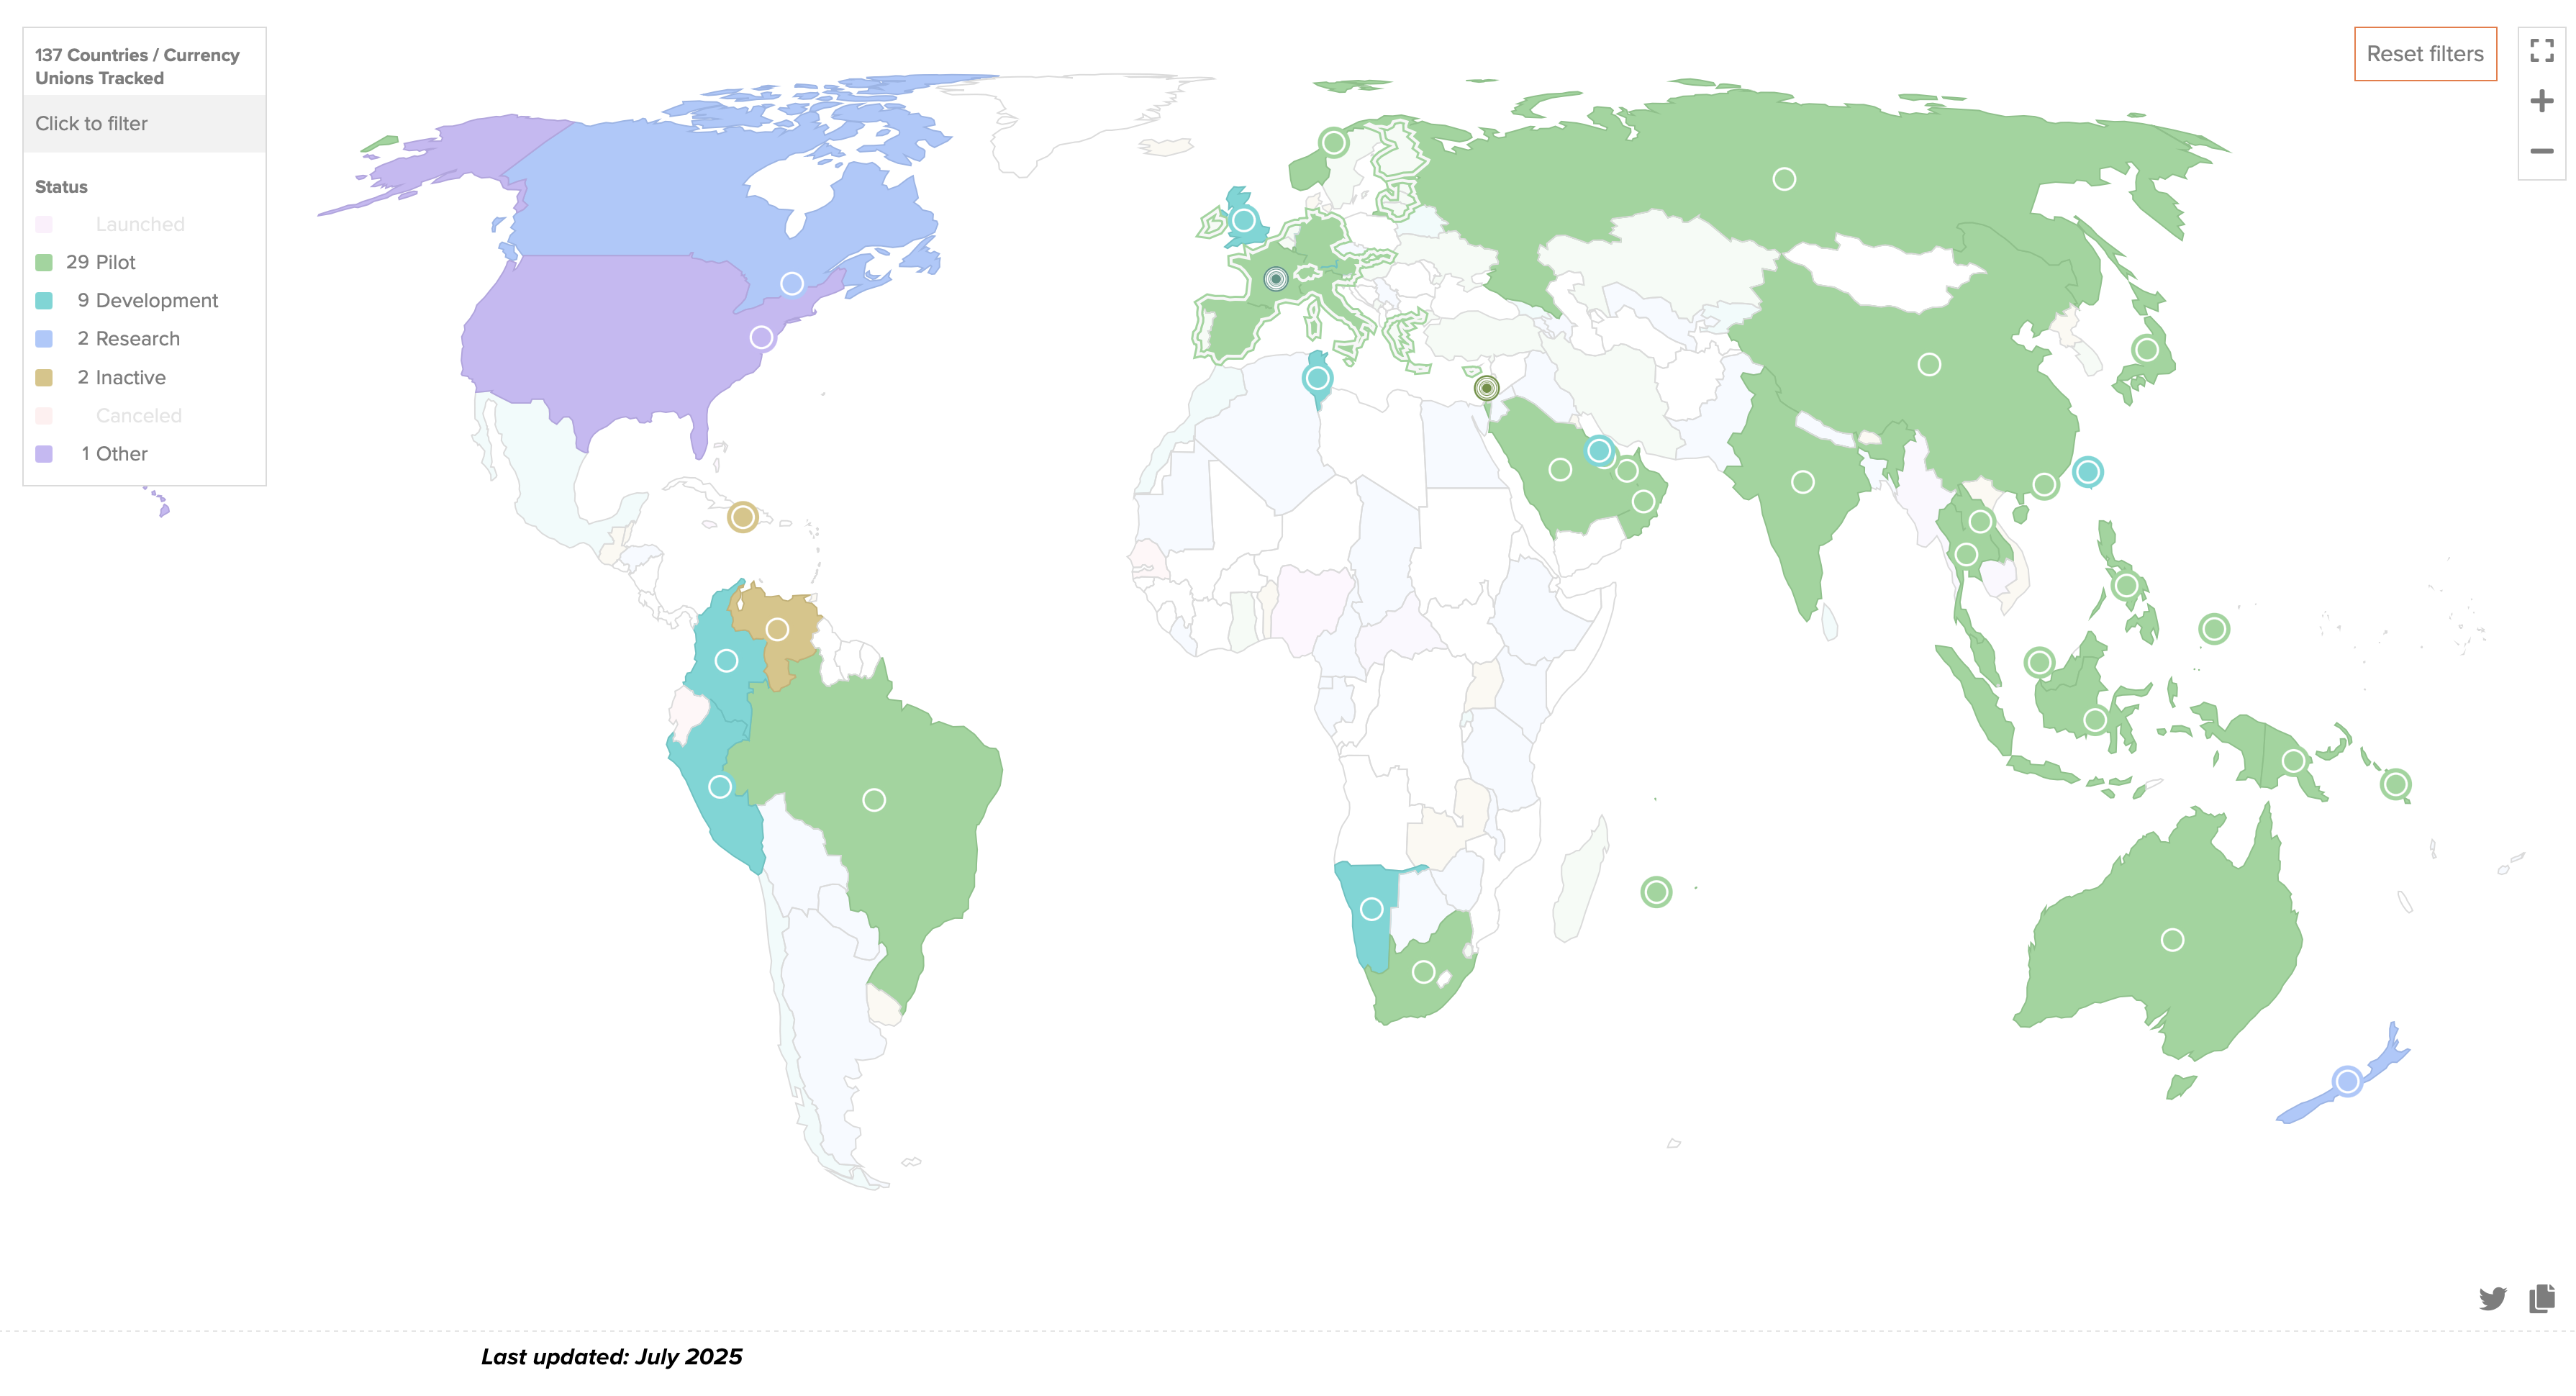
\includegraphics[width=1\linewidth]{Figures/CBDC Wholesale.png}
    \caption{Major wholesale CBDC experiments worldwide. Source: BIS Innovation Hub; Atlantic Council CBDC Tracker.}
    \label{fig:CBDC wholesale}
  \end{figure}
\end{frame}

\begin{frame}{Will Wholesale CBDCs Replace Banking?}
  \textbf{Arguments for:}
  \begin{itemize}
    \item Correspondent banking is expensive, slow, and increasingly fragile
    \item Wholesale CBDCs could reduce settlement time from days to seconds
    \item Direct central bank money eliminates credit risk
    \item Programmable payments (smart contracts) could automate compliance, FX conversion, and reporting
  \end{itemize}
  
  \vspace{0.5em}
  \textbf{Arguments against:}
  \begin{itemize}
    \item \bad{Geopolitical complexity}: Sharing financial infrastructure across countries requires deep political trust. 
    \item \bad{Governance}: Who controls the shared platform? Whose rules apply?
    \item \bad{AML/KYC}: Faster payments make it harder to screen for illicit transactions. %Regulators may resist speed if it comes at the cost of compliance.
    \item \bad{Incumbents}: SWIFT has launched its own modernisation. The existing system is improving, reducing the urgency for replacement.
  \end{itemize}
  
  \vspace{0.3em}
  Wholesale CBDCs are the most promising institutional blockchain application, but deployment at scale is years away.
\end{frame}

%----------------------------------------------------------------------------------------
\section{Public vs.\ Permissioned: The Strategic Question}
%----------------------------------------------------------------------------------------

\begin{frame}{Two Visions of Blockchain in Finance}
  The financial industry is divided on a fundamental strategic question: should institutional blockchain infrastructure be built on \highlight{public} or \highlight{permissioned} networks?
  
  \begin{center}
    \small
    \begin{tabular}{p{2cm}p{4cm}p{4cm}}
      \toprule
      & \textbf{Public} (e.g., Ethereum) & \textbf{Permissioned} (e.g., Kinexys, Canton) \\
      \midrule
      Access & Open to anyone & Approved participants only \\
      Consensus & PoS / PoW (trustless) & Simple agreement (trusted nodes) \\
      Privacy & Transactions visible & Configurable privacy \\
      Composability & High (any protocol can interact) & Low (siloed by design) \\
      Regulatory comfort & Lower & Higher \\
      Speed & Variable (depends on congestion) & Fast (fewer participants) \\
      Examples & BlackRock BUIDL, Aave & JPMorgan Kinexys, DTCC Ion \\
      \bottomrule
    \end{tabular}
  \end{center}
\end{frame}

\begin{frame}{The Case for Public Chains}
  \textbf{Why some institutions are building on Ethereum:}
  \begin{itemize}
    \item \textbf{Network effects}: Ethereum has the largest developer ecosystem, the most deployed smart contracts, and the deepest liquidity pools. Building on Ethereum means access to this ecosystem.
    \item \textbf{Composability}: A tokenized Treasury bill on Ethereum can be used as collateral in a DeFi lending protocol, creating new financial products that are impossible in siloed permissioned systems.
    \item \textbf{Neutrality}: No single company controls Ethereum. For competing banks, neutrality may be preferable to a platform owned by a rival.
    \item \textbf{Proven security}: Ethereum has secured hundreds of billions of dollars in value for years. Its security model is battle-tested.
  \end{itemize}
  
  \vspace{0.5em}
  \textbf{The strongest example}: BlackRock's BUIDL fund (tokenized T-bills on Ethereum). The world's largest asset manager chose a public blockchain over any private alternative.
  
  \vspace{0.3em}
  \textbf{Limitation}: Public chains are transparent by default. Banks need privacy for many transactions, which requires additional layers.
\end{frame}

\begin{frame}{The Case for Permissioned Chains}
  \textbf{Why most banks still prefer private networks:}
  \begin{itemize}
    \item \textbf{Regulatory clarity}: Regulators are more comfortable with identifiable, accountable participants than with open networks.
    \item \textbf{Privacy}: Banks cannot have their trading activity visible to competitors on a public ledger.
    \item \textbf{Performance}: Permissioned chains are faster and more predictable (no gas fees, no congestion from unrelated transactions).
    \item \textbf{Control}: If something goes wrong, there is a governance structure that can intervene. On a public chain, there is no one to call.
  \end{itemize}
  
  \vspace{0.5em}
  \textbf{Limitation}: Permissioned chains are often little more than shared databases with blockchain branding. If only four banks share a ledger, the decentralisation benefit is minimal.
  
  \vspace{0.5em}
  \begin{block}{The Key Question}
    Does putting financial infrastructure ``on blockchain'' genuinely improve outcomes, or is it a technology solution in search of a problem? The answer depends on the specific use case and the number of participants.
  \end{block}
\end{frame}

\begin{frame}{The Likely Outcome: Hybrid Architectures}
  The emerging consensus is that neither pure public nor pure permissioned chains will dominate. Instead, institutions are likely to adopt \highlight{hybrid} architectures:
  
  \vspace{0.5em}
  \begin{itemize}
    \item \textbf{Public chains for settlement and composability}: Assets issued on Ethereum (or similar) for access to global liquidity and DeFi integration.
    \item \textbf{Permissioned layers for privacy and compliance}: KYC-verified ``pools'' or Layer 2 networks where only approved parties can transact, built on top of public chains.
    \item \textbf{Bridges and interoperability protocols}: Connecting different chains so that a tokenized bond on Canton can interact with cash on Fnality or collateral on Ethereum.
  \end{itemize}
  
  \vspace{0.5em}
  \textbf{Analogy}: The internet is a public network, but companies build private intranets and VPNs on top of it. The same pattern may emerge for financial blockchains.
  
  \vspace{0.3em}
  \textbf{The risk}: Interoperability is hard. Cross-chain bridges have been the source of some of the largest hacks in crypto history.
\end{frame}

%----------------------------------------------------------------------------------------
\section{Integration Challenges and Reality Check}
%----------------------------------------------------------------------------------------

\begin{frame}{The ``Last Mile'' Problem}
  Even if blockchain technology works perfectly, integrating it into existing financial infrastructure is enormously difficult.
  
  \vspace{0.5em}
  \textbf{Legacy system compatibility:}
  \begin{itemize}
    \item Banks run on systems built decades ago (many still use COBOL, a programming language from the 1960s)
    \item New blockchain systems must interface with these legacy platforms during any transition
    \item Running old and new systems in parallel is expensive and complex
  \end{itemize}
  
  \vspace{0.5em}
  \textbf{Legal recognition:}
  \begin{itemize}
    \item When is a blockchain transaction legally final? Most legal systems were designed for paper-based or centralised electronic settlement.
    \item The UK Law Commission (2023) recommended recognising digital assets as property---a positive step, but still limited legislation.
    \item EU's DLT Pilot Regime (2023) allows limited use of DLT for securities issuance and settlement under a regulatory sandbox.
  \end{itemize}
  
  \vspace{0.3em}
  \textbf{Coordination problem}: No single bank can switch to blockchain settlement alone. A classic \highlight{network effect} problem with a chicken-and-egg dynamic.
\end{frame}

\begin{frame}{A Sober Assessment of Timelines}
  \textbf{What is realistic?}
  
  \vspace{0.5em}
  \textbf{Already happening} (deployed, live usage):
  \begin{itemize}
    \item Tokenized treasuries and money market funds (BlackRock BUIDL, Franklin Templeton)
    \item Intraday repo and interbank payments (JPMorgan Kinexys)
    \item Pilot programmes for securities settlement (DTCC, SIX Digital Exchange in Switzerland)
  \end{itemize}
  
  \vspace{0.5em}
  \textbf{Plausible within 3--5 years}:
  \begin{itemize}
    \item Broader tokenized bond markets
    \item Wholesale CBDC systems in selected corridors
    \item More asset managers issuing on public blockchains
  \end{itemize}
  
  \vspace{0.5em}
  \textbf{Unlikely within 5 years}:
  \begin{itemize}
    \item Full replacement of existing settlement infrastructure
    \item Global interoperable CBDC network
    \item Equities settling on-chain at scale
  \end{itemize}
  
\end{frame}

%----------------------------------------------------------------------------------------
\section{Summary and Next Steps}
%----------------------------------------------------------------------------------------

\begin{frame}{Key Takeaways}
  \begin{enumerate}
    \item \textbf{Traditional settlement is slow and costly by design}
    \begin{itemize}
      \item Multiple intermediaries, separate records, T+1 delays
      \item But netting provides real economic value that instant settlement would lose
    \end{itemize}
    
    \vspace{0.3em}
    \item \textbf{Institutional blockchain initiatives are real but narrow}
    \begin{itemize}
      \item JPMorgan Kinexys, DTCC Ion, Canton, Fnality---each solves a specific problem
      \item Most are closed systems with limited participants
    \end{itemize}
    
    \vspace{0.3em}
    \item \textbf{Wholesale CBDCs could transform cross-border payments}
    \begin{itemize}
      \item Correspondent banking is ripe for disruption
      \item But geopolitics, governance, and compliance create barriers
    \end{itemize}
    
    \vspace{0.3em}
    \item \textbf{Public vs.\ permissioned is a false dichotomy}
    \begin{itemize}
      \item Hybrid architectures are the likely outcome
      \item Public for settlement and composability; permissioned for privacy and compliance
    \end{itemize}
    
    \vspace{0.3em}
    \item \textbf{The biggest barrier is integration, not technology}
    \begin{itemize}
      \item Legacy systems, legal recognition, and coordination problems matter more than blockchain performance
    \end{itemize}
  \end{enumerate}
\end{frame}

\begin{frame}{What's Next}
  \textbf{Course Synthesis and Future Trends}
  \begin{itemize}
    \item Interoperability and cross-chain bridges
    \item AI and blockchain: synergies and limitations
    \item The future of money: stablecoins, CBDCs, and crypto coexistence
    \item Career paths in blockchain and digital assets
    \item Course synthesis and exam preparation
  \end{itemize}
  
  \vspace{1em}
  \textbf{Preparation:}
  \begin{itemize}
    \item Think about: What problems in finance \textit{genuinely} need blockchain, and which could be solved more simply with better databases?
    \item Reflect: Across the entire course, which blockchain applications have the strongest economic case, and which are solutions in search of a problem?
  \end{itemize}
\end{frame}

\begin{frame}[plain]
  \vfill
  \begin{center}
    {\Large Questions?}
  \end{center}
  \vfill
\end{frame}

\end{document}